% Preamble
% ---
\documentclass[11pt, listof=totoc]{scrreprt}

% Packages
% ---
\usepackage[utf8]{inputenc} % Unicode support (Umlauts etc.)
\usepackage{float}
\usepackage[ngerman]{babel} % Change hyphenation rules
\usepackage[autostyle=true, german=quotes]{csquotes}
\newcommand{\q}[1]{\enquote{#1}}
\usepackage{graphicx} % Add pictures to your document
\usepackage{listings} % Source code formatting and highlighting

%Layout
\usepackage[left=2.5cm, right=2.5cm, top=2cm, headsep=0cm]{geometry}
\usepackage[onehalfspacing]{setspace} %singelspacing

% Schusterjungen und Hurenkinder vermeiden
\clubpenalty = 10000
\widowpenalty = 10000
\displaywidowpenalty = 10000

%KOPF UND FUßZEILE%%%%%%%%%%%%%%%%%%%%%%%%%%%%%%%
\usepackage{scrlayer-scrpage}
\pagestyle{scrheadings}
\renewcommand*\chapterpagestyle{scrheadings}
\clearscrheadfoot

%Kopfzeile
\ihead{\setstretch{1}{\begin{large}\textsc{Charaktersteuerung}\\\end{large}
\begin{small}
Programmierung einer intuitiven Charaktersteuerung\\
\end{small}
\vspace{7pt}
\leftmark}}
\automark{chapter}
\ohead{
\includegraphics[scale=0.25]{Bilder/ckc_logo.png}}
\setheadsepline{1pt}

%Fußzeile
\ifoot{Marvin Jung}
\ofoot{
\begin{large}
\thepage
\end{large}}

%Abstand über und unter Kapitel
\setlength{\headsep}{16pt}
\RedeclareSectionCommand[beforeskip=0pt, afterskip=8pt]{chapter}


%Quellenverzeichnis
\usepackage[backend=bibtex, sorting=none]{biblatex}
\bibliography{Quellen}
\newcommand{\fcitetitle}[1]{\footnote{\citetitle{#1} [\citefield{#1}{year}] \cite{#1}}}

% Tabellensettings:
\usepackage{xcolor}
\usepackage{tabularx}
\usepackage{colortbl}
\usepackage{textcomp}
\definecolor{ckcGreenDark}{rgb}{0.457,0.523,0.117}
\definecolor{ckcGreen}{rgb}{0.664,0.781,0.156}
\definecolor{odd}{rgb}{0.9,0.9,0.9}
\usepackage{chngcntr}
\counterwithout{table}{section}
\newcommand{\tref}[1]{[\ref{#1}]}

\newcommand{\cc}{$ ^\circ $}
\newcommand{\fullref}[1]{\autoref{#1} \nameref{#1}}


\usepackage[nottoc]{tocbibind}
\usepackage[linktocpage=true, colorlinks=true, 
linkcolor=ckcGreenDark, citecolor=ckcGreenDark, urlcolor=ckcGreenDark
%linkcolor=black, citecolor=black, urlcolor=black
]{hyperref}

%%%%%%%%%%%%%%%%%%%%%%%%%%%%%%%%%%%%%%%%%%%%%%%%%%
%DOKUMENTSTART
%%%%%%%%%%%%%%%%%%%%%%%%%%%%%%%%%%%%%%%%%%%%%%%%%%
\begin{document}

\pagenumbering{gobble} %schaltet die Seitenzahl aus (gobble-keine Zahlen; arabic-zahlen; roman-roman zahlen)

\begin{titlepage}
\begin{center}
\begin{figure}
\centering

\includegraphics[scale=0.05]{Bilder/ihk_logo.png}
\end{figure}
\large
Abschlussarbeit Sommer 2016\\
\vspace{12pt}
Fachinformatiker für Anwendungsentwicklung\\
\vspace{4pt}
\Large
Dokumentation zur betrieblichen Projektarbeit\\
\vspace{70pt}

\textbf{\huge
Charaktersteuerung\\
\vspace{15pt}
\Large
Programmierung einer intuitiven Charaktersteuerung im Projekt "`Sisyfox"'\\
}
\vspace{22pt}
\small
Abgabetermin: 26.04.2016\\
\vspace{28pt}
\normalsize
\textbf{Prüfungsbewerber:\\}
Marvin Jung\\
Weddinger Str. 23\\
38690 Immenrode\\
\vspace{30pt}
\begin{figure}[ht]
\centering

\includegraphics[scale=0.6]{Bilder/ckc_logo.png}
\end{figure}
\textbf{Ausbildungsbetrieb:\\}
ckc ag\\
Am Alten Bahnhof 13\\
38122 Braunschweig\\

\end{center}
\end{titlepage}

\newpage{}

\pagenumbering{Roman}
\tableofcontents{} %generiert das Inhaltsverzeichnis
\addtocontents{toc}{~\hfill\textbf{Seite}\par}
\newpage{}
\listoffigures
\listoftables
\newpage{}
\pagenumbering{arabic} %schaltet die Seitenzahl ein

\chapter{Einleitung}
\paragraph{}
Die ckc group ist ein von Christian Krentel im Jahr 1989 gegründeter IT- und Business-Consulting-Anbieter in Braunschweig. Sie gehört in dem Bereich zu den führenden Unternehmen Deutschlands. In den Standorten Braunschweig, Berlin, Darmstadt, Hamburg, Dortmund und München beschäftigt sie rund 400 Mitarbeiter\fcitetitle{Mitarbeiterzahl}.
\paragraph{}
Hauptbranchen des Unternehmens sind die Automobilindustrie samt Zulieferer sowie Banken, Versicherungen, Luft- und Raumfahrt, Retail, Transport und Logistik. Die Kernkompetenz von ckc liegt im Bereich der IT nicht nur auf der 
Softwareentwicklung, sondern zu Teilen zusätzlich auf der Managementberatung.

\section{Projektbeschreibung}
\paragraph{}
Das ”Sisyfox” Projekt wird entworfen, um für firmeninterne Events (z.B. Seminare, Konferenzen, Sommerfeste, etc.) eine Attraktion zu bieten, die nicht nur mit Spaß verbunden wird, sondern aus der sich auch ein Lernwert ergibt. 
Das Spiel stellt in einer vereinfachten Form den Mythos des Sisyphos und sein immerwährendes Scheitern gamifiziert\fcitetitle{Gamifizierung} dar. Den Mitarbeitern soll dabei der Umgang mit dem Erlebnis des Scheiterns näher gebracht werden. Außerdem soll diese Gamifizierung zu einer Motivationssteigerung führen.
\paragraph{}
Der Charakter im Spiel wird mit einem Aufbau, auf dem ein 1.20m großer Ball als Steuerkugel\footnote{Wie in einem Kugellager.} befestigt ist, vom Spieler gelenkt. Dafür steht der Aufbau vor dem Spieler auf dem Boden. 
Die Kugel kann durch den Aufbau mit den Händen auf der Stelle bewegt werden. Die Sensordaten des Aufbaues werden direkt an den Computer übermittelt und müssen in der Steuerung umgesetzt werden. 
\paragraph{}
Meine Aufgabe in dem Projekt besteht darin, die Steuerung für den Charakter im Spiel zu programmieren. Diese wird in der Programmiersprache C\# geschrieben, damit sie in der Spieleentwicklungsumgebung ”Unity” als Skript in das vorhandene Projekt eingebunden werden kann. Hierbei muss auf eine intuitive Steuerung geachtet werden, da die Attraktion einer großen Zielgruppe zur Verfügung gestellt werden soll. Im Projekt vorhanden sind bereits sämtliche Modelle, Animationen, sowie Sounds und Hintergrundmusik, aber auch schon einzelne, von mir früher programmierte Skripte, die sich z.B. um das Benutzerinterface kümmern. Die benötigten Daten für die Steuerung des Charakters werden von einer Trackballmaus zum Computer übertragen und müssen dort in die Bewegung umgesetzt werden. Außerdem muss im Rahmen der Projektarbeit bestimmt werden, wie sich der Charakter in der virtuellen Welt verhält, sowie in welchen Situationen der Spieler das Spiel vorzeitig verlieren kann und ab welchem Zeitpunkt das Spiel gewonnen ist.

\section{Projektziel}
\paragraph{}
Mit dem Projekt möchte ich eine gewisse Hartnäckigkeit, gefolgt von gesteigerter Motivation durch Erfolgserlebnisse bei den Mitarbeitern, sowie Besuchern von Firmenfesten und anderen Events erzielen. Der Benutzer wird mit jeder gespielten Runde vor die Aufgabe gestellt eine scheinbar unerreichbare Hürde zu überwinden. Er wird viele Versuche brauchen, um den Gipfel zu erreichen. Der spielerische Aspekt sorgt unweigerlich dafür, dass der Benutzer leichter mit häufigen Niederlagen umgehen kann, um anschließend den anfangs weit entfernten Berg erneut herauszufordern. Sobald der Spieler am Gipfel angekommen ist, gibt es auditive und visuelle Erfolgsmeldungen. Dazu kommt eine Anzeige, wie lange der Weg zur Bergspitze gedauert hat, damit der Spieler sich mit anderen messen kann und ein Wettkampfgefühl entsteht.

\section{Projektabgrenzung}
\label{Projektabgrenzung}
\paragraph{}
Im Projekt sind bereits ein Spielehauptcontroller, sowie ein Animations- und Bewegungssteuerung vorhanden.
Der Hauptcontroller sorgt für die Verwaltung der Grundstatus\footnote{Die vier Status sind inaktiv, spielend, gewonnen und verloren.} im Spiel. Außerdem speichert er die wichtigsten Variabeln, wie unteranderem Spieldauer oder die Höhe abweichend vom Fuß des Berges. Es wird lediglich ein Verweis via Assoziation in der Charaktersteuerung eingebunden.

\chapter{Projektplanung}
\section{Projektphasen}
\paragraph{}
Für die Umsetzung des Teils des Projekts stehen insgesamt 70 Stunden zur Verfügung. Die Softwareentwicklung wurde vor Beginn des Projekts auf die verschiedene Projektphasen aufgeteilt. In der folgenden Tabelle \tref{tab:Zeit} lässt sich die grobe Zeitplanung ablesen.\\
\begin{table}[h]
\centering
\begin{tabular}{lr}
\rowcolor{ckcGreen}\textbf{Projektphase} & \textbf{Geplante Zeit}\\
\hline
Ist-Analyse & 6 Std\\
\rowcolor{odd}Soll-Konzept & 11 Std\\
Implementierung & 24 Std\\
\rowcolor{odd}Integration in das Unityprojekt &  8 Std\\
Testen und Fehlerbehebung & 11 Std\\
\rowcolor{odd}Dokumentation & 10 Std\\
\hline
\hline
\rowcolor{ckcGreen}\textbf{Gesamt} & \textbf{70 Std}\\
\end{tabular}
\caption{Grobe Zeitplanung}
\label{tab:Zeit}
\end{table}
\paragraph{}
Eine verfeinerte Version, in der die einzelnen Hauptphasen noch untergliedert sind, befindet sich im Anhang \textit{Anhangsverweis einfügen} auf der Seite \textit{Seitenzahl einfügen}.

\section{Ressourcenplanung}

\chapter{Analysephase}
\section{Ist-Analyse}
In dem Spiel gibt es viele kleine Details, welche über das Einbinden von Scripten und das Platzieren von 3D-Modellen realisiert werden. Dazu gehört zunächst die Spielkarte auf der sich der Charakter bewegt. Diese wurde von anderen Teammitgliedern erstellt, mit 3D-Modellen wie z.B. Bäumen, Sträuchern oder Gesteinsbrocken bestückt und in das Projekt implementiert. Zusätzlich wurden 3D-Modelle von Wolken und Vögeln erstellt, die sich im Kreis um den Hauptberg bewegen\footnote{Die Bewegung wurde mit einem Script realisiert.}.
Der Spielecharakter namens \q{Sisyfox} gehört zu den schon erstellten 3D-Modellen und wurde ebenfalls schon mit einer vollständiger Animation versehen.
Wie in Sektion \ref{Projektabgrenzung} (Projektabgrenzung) schon angedeutet ist der Hauptcontroller, als einer von vielen Scripten, schon vorhanden. Weitere wichtige Scripte sind die Kamerasteuerung, sämtliche Animationsscripte, eine Höhenmeteranzeige und ein Arduinokommunikationsscript, welcher eine Verbindung zu einer Hardwarekonstruktion namens \q{Arduino\fcitetitle{Arduino}} aufbaut. Letzter sorgt dafür, dass sich relativ zur Höhe auf der sich der Charakter befindet, ein angeschlossener Ventilator stärker dreht und eine Nebelmaschine kurz vor Erreichen des Gipfels anspringt.
Um das Spiel zu komplettieren fehlt nun die Charaktersteuerung. 

\section{Anwendungsfälle}

\chapter{Entwurfsphase}
\section{Zielplattform}
\section{Architekturdesign}
\section{Entwurf der Benutzeroberfläche}
\section{Geschäftslogik}
\section{Maßnahmen zu Qualitätssicherung}

\chapter{Implementierungsphase}
\section{Implementierung der Benutzeroberfläche}
\section{Implementierung der Geschäftslogik}

\chapter{Abnahme- und Einführungsphase}

\section{Abnahme}
\section{Einführung}
\section{Dokumentation}

\chapter{Fazit}
\section{Soll- / Ist-Vergleich}
\section{Lessons Learned}
\section{Ausblick}


\printbibliography[heading=bibintoc,title={Literaturverzeichnis}]
\newpage{}

\appendix
\pagenumbering{roman}
\chapter{Anhang}

\begin{figure}[H]
\centering
\caption{Benutzer Oberfläche Skizze}
\label{Abb:UISkizze}
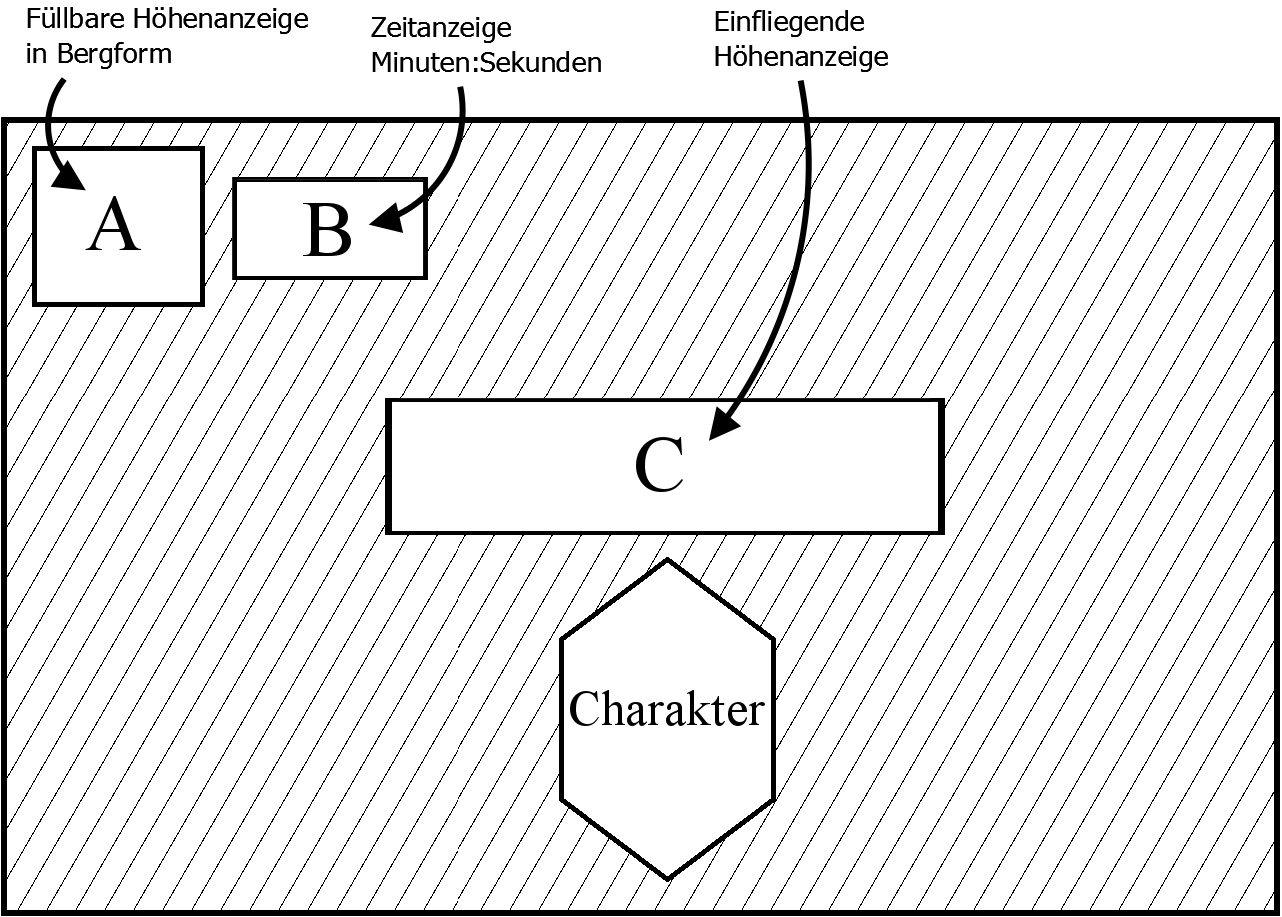
\includegraphics[scale=0.285]{Bilder/Diagramme/UserInterface.png}

\caption{Benutzer Oberfläche Im Spiel}
\label{Abb:UIIngame}
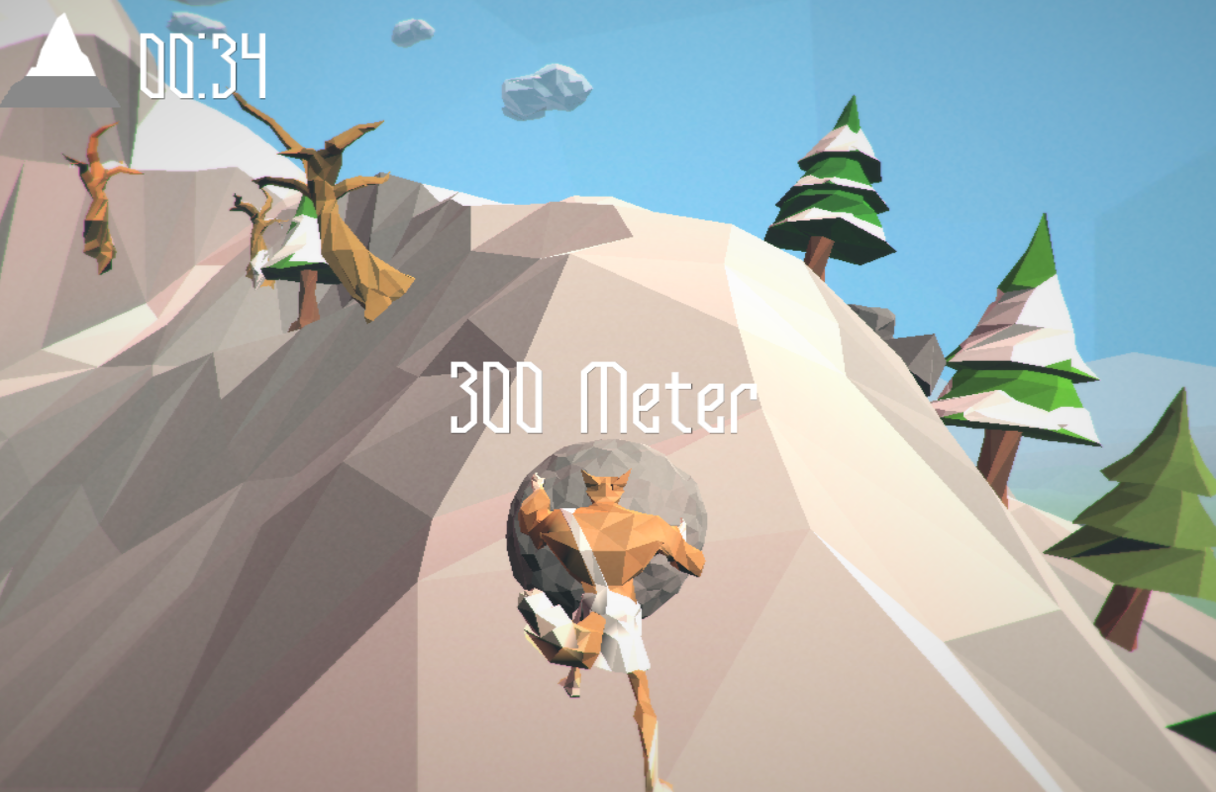
\includegraphics[scale=5.25]{Bilder/SisyfoxUI.png}
\end{figure}
\newpage{}

\begin{figure}[H]
\raggedright
\caption{Verwendete Ressourcen}
\label{Abb:Ressourcen}
\textbf{Hardware:}
\begin{itemize}
\item Büroarbeitsplatz mit Standrechner
\end{itemize}
\textbf{Software:}
\begin{itemize}
\item Windows 7 Professional Service Pack 1 - Betriebssystem
\item Unity 3D Version 5.3.3f1 - 3D Entwicklungsumgebung
\item Visual Studio 2015 - Code Entwicklungsumgebung
\item MiK\TeX - Distribution des Textsatzsystems \TeX
\item \TeX{}Maker - \LaTeX Schreibprogramm
\item Dia Version 0.97.2 - Anwendung zum Zeichnen strukturierter Diagramme
\end{itemize}
\begin{itemize}
\item Entwickler - Implementierung der Scripte / Realisierung
\item Anwendungsentwickler - Code Begutachtung
\end{itemize}
\end{figure}


\begin{figure}[H]
\centering
\caption{Model View Controller}
\label{Abb:MVC}
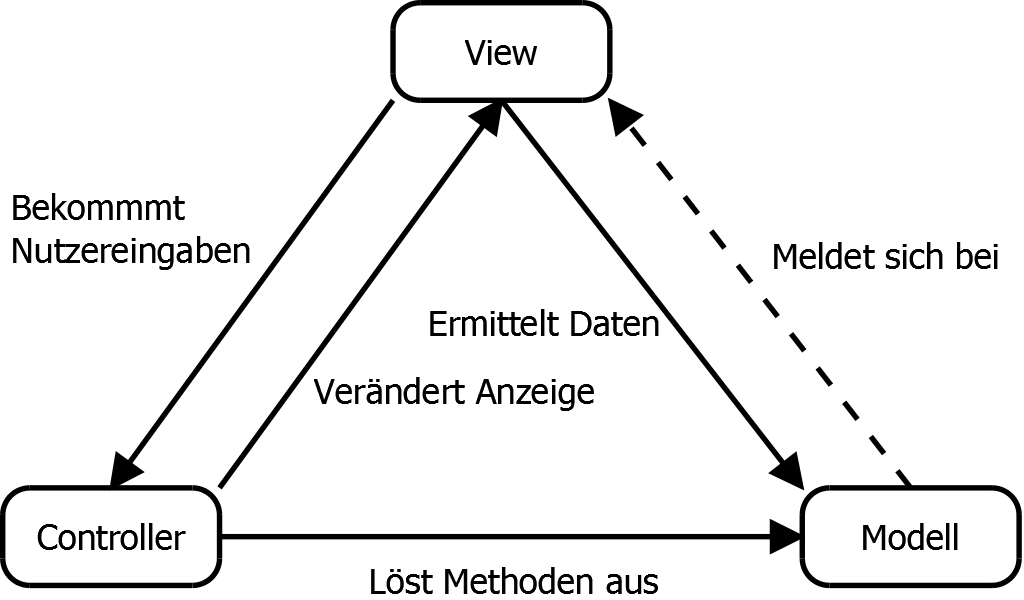
\includegraphics[scale=0.5]{Bilder/Diagramme/MVC.png}
\end{figure}

\begin{figure}[H]
\centering

\caption{Presentation Abstraction Control}
\label{Abb:PAC}
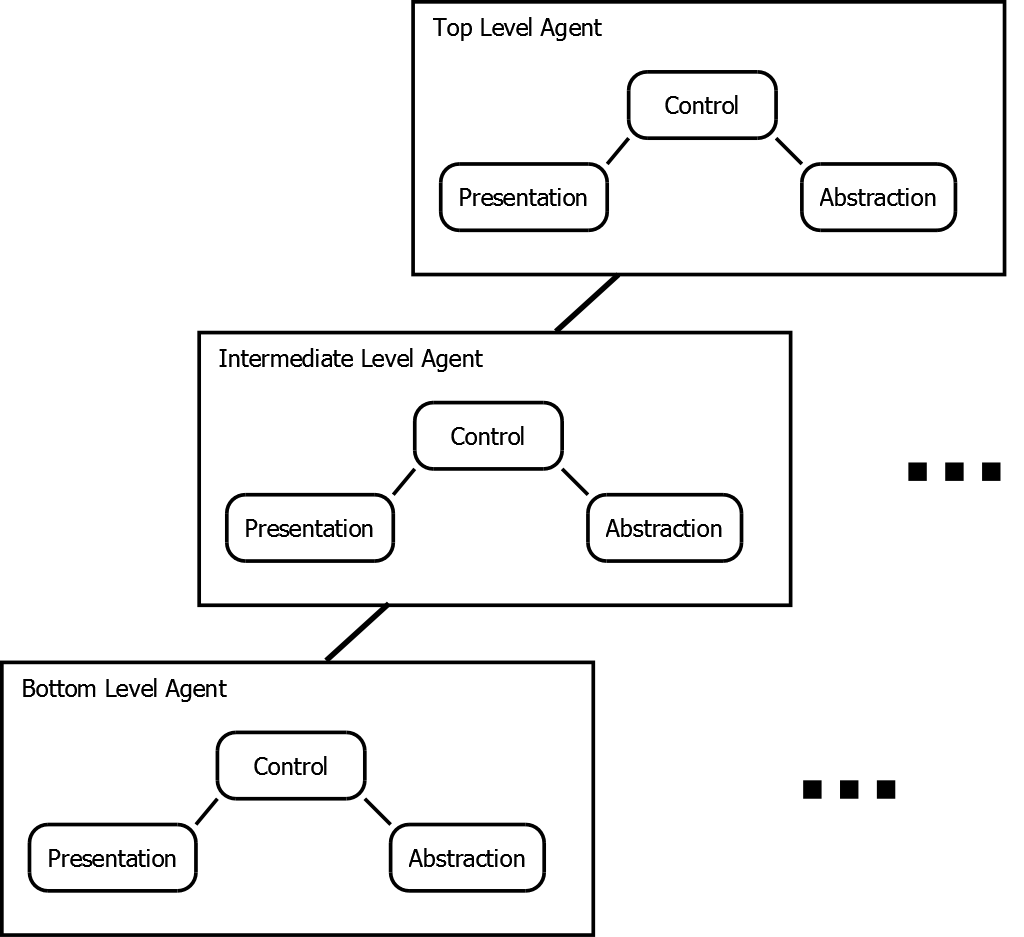
\includegraphics[scale=0.275]{Bilder/Diagramme/PAC.png}
\end{figure}

\begin{figure}[H]
\centering
\caption{Klassendiagramm Charaktersteuerung mit Sphere}
\label{Abb:KlassendiaMain}
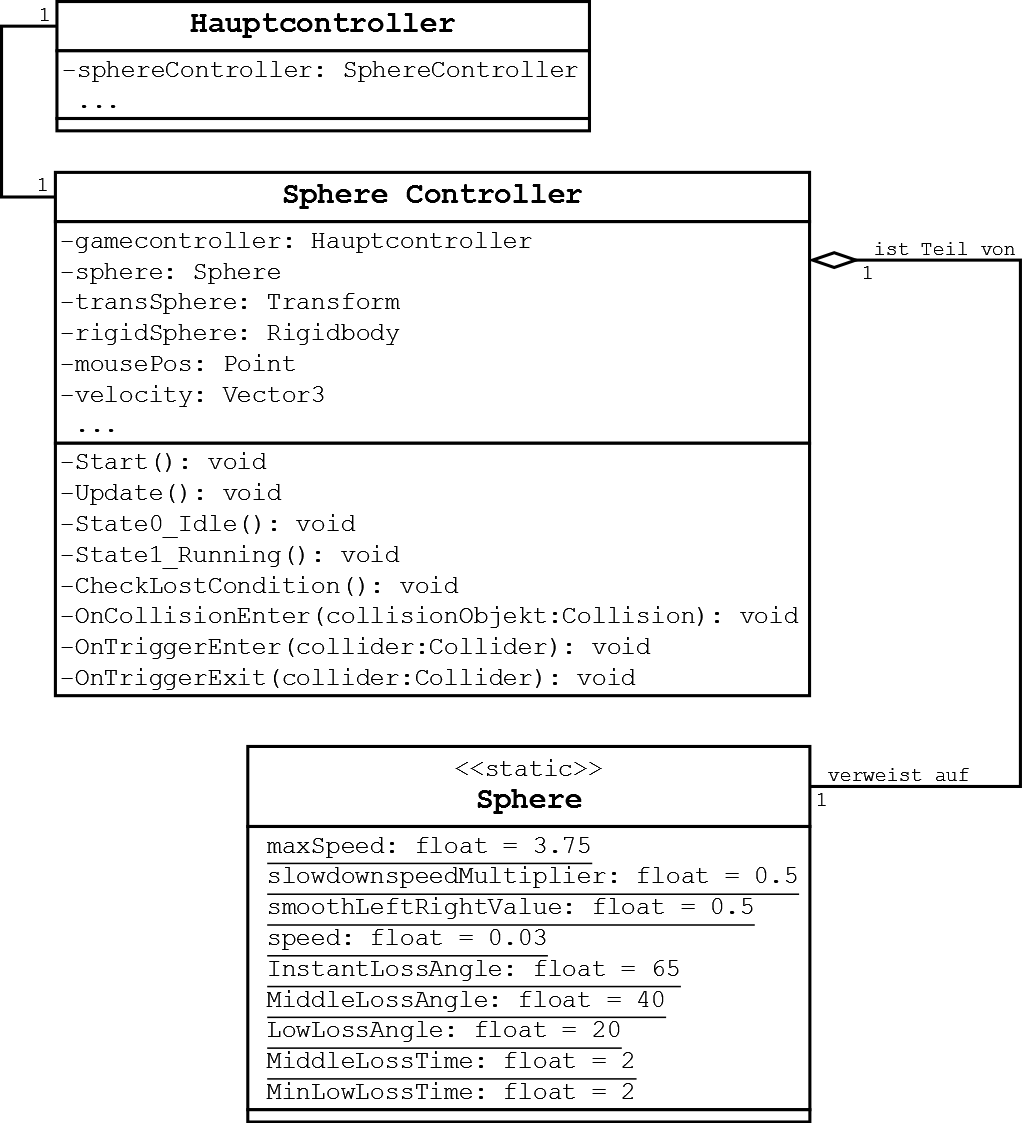
\includegraphics[scale=0.3]{Bilder/Diagramme/KlassendiagrammMain.png}
\end{figure}

\begin{figure}[H]
\centering
\caption{Zustandsdiagramm Statusverwaltung}
\label{Abb:SMStatus}
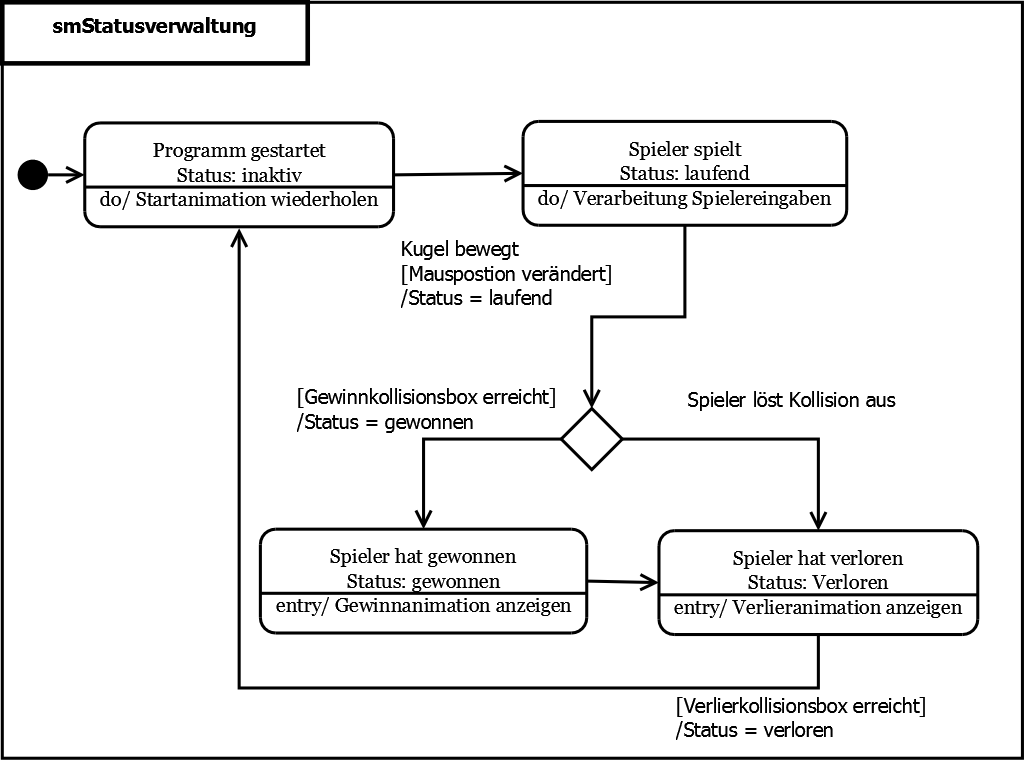
\includegraphics[scale=0.35]{Bilder/Diagramme/smStatusverwaltung.png}
\end{figure}

\begin{figure}[H]
\centering
\caption{Verloren Status bei seitlichem Steigungswinkel}
\label{Abb:SeitlWinkel}
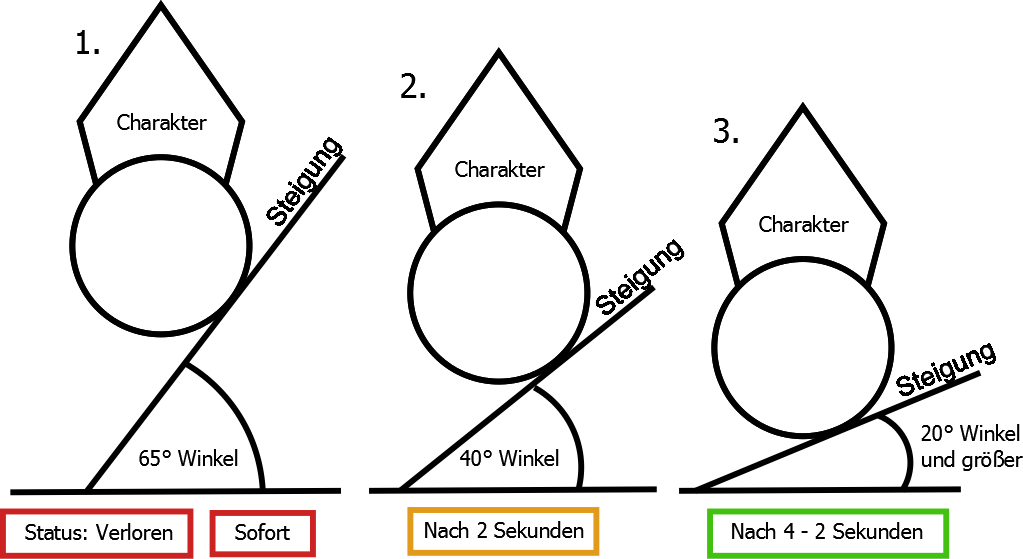
\includegraphics[scale=0.275]{Bilder/Diagramme/VerlierWinkelSeitlich.png}
\end{figure}


\end{document}
